\documentclass[12pt]{article}
\usepackage[top=1in, bottom= 1in, left= 1in, right= 1in]{geometry}
\usepackage[USenglish]{babel} % set the language; greek allows \textgreek{\euro}
\usepackage{multirow} % For tables
\usepackage{graphicx, subfigure} % For graphics
\usepackage{fancyhdr} % Produces fancy headers
\usepackage{setspace} % allows for vsape
\usepackage{natbib} % package to organize literature --> google it!
\usepackage{verbatim} % For including R-code
\usepackage{booktabs} % nicer tables
\usepackage{alltt} % verbatim + highlighting
\usepackage{amsmath} %boldsymbols
\usepackage{lscape} %Querformat
\usepackage{dcolumn} % align at decimal mark
\usepackage{floatrow} % description paragraphs below figures and tables
\usepackage{enumerate} % alter enumerate items (i,ii,iii etc)
\usepackage[title]{appendix} % enumerated appendices etc.
\usepackage{xcolor}
\usepackage{todonotes}
\usepackage[colorlinks=true,citecolor=red!50!black,urlcolor=blue!50!black,linkcolor=red!50!black]{hyperref}
\setlength{\headheight}{15pt}
% http://en.wikibooks.org/wiki/LaTeX/Page_Layout for additional info

\author{Patrick W. Kraft\footnote{PhD Student, Stony Brook University, \href{mailto:patrick.kraft@stonybrook.edu}{patrick.kraft@stonybrook.edu}}}
\date{today}

\title{Moral Foundations of Political Reasoning\footnote{Draft in preparation for the 2015 Annual Conference of the Midwest Political Science Association, comments welcome!}\\
\large{Investigating the Moral Underpinnings of Political Judgment}}
\date{\today}


\begin{document}
\maketitle

\begin{abstract}%\onehalfspacing
According to Moral Foundations Theory, moral thinking is fundamentally structured by five central innate intuitions \citep{haidt2008moral}. Furthermore, as \citet{graham2009liberals} showed in a subsequent set of studies, liberals and conservatives rely on different sets of moral foundations \citep[see also][]{haidt2007morality}. The goal of the paper presented here is to extend the analyses conducted by \citet{graham2009liberals} and investigate whether individuals actually rely on moral foundations when evaluating political candidates and parties. Based on open-ended survey responses in the 2012 American National Election Study, it will be examined to what extent the apparent differences in moral judgments between liberals and conservatives actually shape and structure individual reasoning and evaluations in the political context. More specifically, I utilize the moral word lists used by \citet{graham2009liberals} in the context of sermons to identify references to basic moral intuitions when individuals report on their attitudes towards political parties and candidates. Consistent with \citet{graham2009liberals}, it is hypothesized that liberals and conservatives differ with regard to the set of moral foundations they rely on when evaluating political actors. Furthermore, it will be investigated whether these relationships connecting ideology and moral reasoning are moderated by political interest or expertise. The results indicate that moral values can indeed be seen as determinants of ideological thinking, rather than only being a rhetorical device that citizens learn to bolster their political views.

\noindent \textbf{keywords} Moral Foundations Theory, Political Ideology, Political Reasoning, Open-ended Survey Responses
\end{abstract}

\newpage
\singlespacing

\section{Introduction}

A growing body of literature in political science and psychology investigates basic individual characteristics and underlying motivations that shape political belief systems and ideologies \citep[c.f.][]{jost2003political,jost2006end,jost2009political}. For example, it has been shown that liberals and conservatives differ with regard to their personality dimensions \citep{gerber2010personality,hirsh2010compassionate,de2013personality}, social values \citep{schwartz2010basic,schwartz2011basic,piurko2011basic}, or moral considerations \citep{lakoff1995metaphor,haidt2008moral,mcadams2008family}. In the domain of morality, \citet{haidt2008moral} presented a model that describes five central innate intuitions that structure moral thinking. In a subsequent set of studies, \citet{graham2009liberals} showed that liberals and conservatives indeed rely on different sets of moral foundations \citep[see also][]{haidt2007morality}. More specifically, the authors found significant differences between liberals and conservatives with regard to self-reported moral judgments. Furthermore, \citet{graham2009liberals} analyzed liberal and conservative sermons and showed that they also diverged with regard to the degree to which they referenced certain moral foundations.

The goal of this paper is to extend the analyses conducted by \citet{graham2009liberals} and investigate whether individuals actually rely on moral foundations when evaluating political candidates and parties. Accordingly, it will be examined to what extent the apparent differences in moral judgments between liberals and conservatives actually shape and structure individual reasoning and evaluations in the political context. The analyses presented in this paper are based on open-ended survey responses in the 2012 American National Election Study. More specifically, I utilize the moral word lists used by \citet{graham2009liberals} in the context of sermons to identify references to basic moral intuitions when individuals report on their attitudes towards political parties and candidates.

Using open-ended questions instead of closed survey responses has important advantages in the context of the research question proposed here. For example, the studies by \citet{graham2009liberals} that focused on self-reported moral judgments convincingly demonstrated systematic patterns of moral reasoning that allowed to differentiate between liberals and conservatives. However, since moral considerations and political beliefs were measured using closed items, it could be argued that these associations are only latent and do not necessarily manifest themselves in actual day-to-day political reasoning. However, showing similar patterns among individuals in a more unobtrusive survey context, where the potential connection between morality and politics is not induced or facilitated by design, could provide stronger evidence for the notion that political reasoning is directly influenced by basic moral intuitions.

Consistent with \citet{graham2009liberals}, it is hypothesized that liberals and conservatives differ with regard to the set of moral foundations they rely on when evaluating political actors. Furthermore, it will be investigated whether these relationships connecting ideology and moral reasoning are moderated by political interest or expertise. The results indicate that moral values can indeed be seen as determinants of ideological thinking, rather than only being a rhetorical device that citizens learn to bolster their political views.

The remainder of the paper is organized as follows: The first section will provide a brief overview over the Moral Foundations Theory laid out by \citet{haidt2008moral}. Subsequently, it will be discussed how moral values and other underlying personal factors determine political ideology. The following part will discuss the role of political reasoning as well as the potential moderating effect of sophistication. The subsequent section will describe the empirical analyses in detail. After presenting the results, the paper concludes with a discussion of potential limitations as well as an outlook for future research avenues.


\section{Theoretical Framework}

\subsection{Moral Foundations Theory}

In one of his influential earlier works on moral psychology, \citet{haidt2001emotional} argued that moral judgment is not based rational reasoning but rather on automatic and affective intuitions, which are in turn influenced by social and environmental factors. More specifically, \citet[825]{haidt2001emotional} described that moral intuition ``appears to be the automatic output of an underlying, largely unconscious set of interlinked moral concepts. These concepts may have some innate basis [...], which is then built up largely by metaphorical extensions from physical experience''. According to this view, explicit moral reasoning can then be better described as a rationalization of these intuitions. \citet{haidt2004intuitive} further developed this view of innateness as a framework to explain cultural differences in moral virtues.

As such, one of the major arguments in the framework of Moral Foundations Theory is the proposition that morality is partially innate, which \citet[367]{haidt2008moral} described as ``organized, to some extent, in advance of experience''. More specifically, \citet{haidt2008moral} identified five basic intuitions which build the psychological foundations of human morality and are inherently linked to evolutionary adaptive challenges that appear cross-culturally. These five basic intuitions are \textit{Harm / Care}, \textit{Fairness / Reciprocity}, \textit{Ingroup / Loyalty}, \textit{Authority / Respect}, and \textit{Purity / Sanctity} \citep[see also][]{graham2011mapping}.\footnote{It is worth noting that later accounts of Moral Foundations Theory discussed the inclusion of further dimensions, such as \textit{Liberty / Oppression} \citep[c.f.][]{graham2013moral,haidt2012righteous}. However, the analyses presented here will only focus on the dimensions initially suggested in \citet{haidt2008moral}.} They represent an innate draft of morality that is further edited by individual experience. This editing process, in turn, is determined by the development of moral virtues as personal characteristics as well as moral narratives \citep{haidt2008moral}.

However, the proposition of innateness of moral judgment was also subject to criticism. For example, \citet{suhler2011can} argued that the definition innateness is essentially too loose and not necessarily backed by the empirical evidence put forward to support it. Rather, \citet{suhler2011can} raised concerns that the theoretical arguments underlying Moral Foundations Theory stand in contrast to recent evidence from neuroscience and genetics.

Irrespective of this theoretical debate about the innateness underlying moral intuitions, numerous research has shown that this theoretical framework provides useful insights in the underlying factors shaping political belief systems and ideologies. As such, we now turn to the discussion of the relationship between moral values and political ideologies.


\subsection{Moral Values and Political Ideology}

Moral and social values have been described as one of the underlying personal characteristics that determine broader political beliefs. For example, \citet{piurko2011basic} described how basic personal values structured underlying motivational meanings of liberal and conservative political orientations \citep[see also][]{schwartz2010basic,schwartz2011basic}. Focusing more closely on moral values, \citet{lakoff1995metaphor} argued that conservative and liberal belief systems can be differentiated by their relative emphasis on specific moral metaphors, namely the strict father model as well as the nurturant parent model. In a subsequent study, \citet{barker2006competing} showed that these nurturant and disciplinarian visions of parental roles can indeed be connected to ideologically coherent views.

As such, the possible connection between moral values and political belief systems also became a major focus in the context of the Moral Foundations framework \citep[c.f.][]{haidt2012righteous}. \citet{haidt2007morality} as well as \citet{graham2009liberals} argued that liberal morals focus on individualizing foundations, which include harm/care and fairness/reciprocity. Conservatives, on the other hand, also emphasize the remaining foundations of ingroup/loyalty, authority/respect, and purity/sanctity, which are labelled as binding foundations. One interesting aspect about their expectations as well as their empirical results is that conservatives do not prioritize less on the individualizing foundations than liberals, but rather that liberals differ in their lower degree of emphasis on binding foundations. Compared to liberals, conservatives tend to endorse and use the five foundations more equally.

\citet{graham2009liberals} presented several empirical analyses to support their hypothesis. More specifically, the authors demonstrated that liberals showed greater endorsement and use of harm/care and fairness/reciprocity foundations when they were asked to evaluate the relevance of moral concerns, when they made explicit moral judgments, as well as in the context of moral trade-offs. Throughout these studies, conservatives endorsed and used the five foundations more equally. The final study presented by \citet{graham2009liberals} consisted of a quantitative analysis of sermons from liberal and conservative churches. The authors proposed a dictionary of words (and word stems) that signal references to the specific moral foundations and showed that liberal sermons where more likely to contain expressions that can be ascribed to the moral foundations of harm/care and fairness/reciprocity. As will be further described below, the analyses presented here will utilize the same dictionary in order to assess moral references in the context of open-ended survey responses.

Overall, these studies strongly support the view that the underlying moral intuitions conceptualized in the Moral Foundations framework differ systematically between liberals and conservatives. While subsequent studies looked more closely at the relationship between moral intuitions and multi-dimensional conceptualizations of ideology \citep[c.f.][]{haidt2009above}, as well as more specific sociopolitical orientations such as social dominance orientation and right-wing authoritarianism \citep[c.f.][]{federico2013mapping}, we will now turn to the question to what extent the connection between moral values and political ideology manifests itself when citizens reason about politics and evaluate political actors.


\subsection{The Role Political Reasoning and Sophistication}

While the research discussed above convincingly showed that liberals and conservatives indeed show different patterns in their emphasis on moral foundations, it is still worth investigating to what degree these considerations differentiate how individuals reason about politics. Indeed, \citet{haidt2008moral} emphasized the importance of moral narratives in the development of moral thinking and \citet{mcadams2008family} showed how conservatives and liberals differed in terms of moral references in life-narrative interviews. But do these moral narratives also shape the political discourse among citizens?

Looking at research on political attitudes and behavior from different perspectives suggests that this is indeed the case. For example, using open-ended survey responses in the context of social welfare attitudes, \citet{feldman1992political} showed that most people makes references to values when they discuss their policy preferences. Looking at the elite level, \citet{clifford2013words} argued that proponents and opponents of stem cell research place distinctive weights on moral foundations which in turn affected the public attitudes and the underlying considerations related to the issue. Furthermore, \citet{clifford2014linking} presented a theory that suggests that individuals rely their own moral motivations in order to interpret and evaluate the behavior of politicians. \citet{marietta2007values} also argued that political value priorities can serve as heuristics for electoral decision-making.

Accordingly, numerous evidence suggests that moral foundations play an important role in the political debate as well as in the evaluation of political actors. Taking into account the fact that moral intuitions (or values in general) appear to play an important role on the elite as well as the electoral level suggests that citizens can be expected to rely on references to moral foundations when reporting on their attitudes towards political actors. Consistent with the arguments and empirical evidence presented by \citet{graham2009liberals} and others, the following hypothesis can be specified:

\vspace{0.3cm}
\begin{tabular}{lp{12cm}}
\textsl{Hypothesis 1:} & Liberals are more likely to emphasize moral foundations of harm/ care and fairness/reciprocity  than conservatives when evaluating political parties and candidates in the context of open-ended survey items. On the other hand, conservatives are more likely to emphasize moral foundations of ingroup/loyalty, authority/respect, and purity/sanctity than liberals.
\end{tabular}
\vspace{0.5cm}

However, one could argue that the hypothesized patterns do not necessarily mean that moral intuitions shape political thinking as such, but rather that they merely serve as a rhetorical device that people learn depending on their political predispositions. However, if this was indeed the case, we could expect that the ideological differences in the emphasis on moral foundations is contingent upon individual levels of political sophistication, interest, and engagement \citep[see also][]{goren2001core,goren2004political}. In other words, political sophistication (or political interest) should moderate the reference to specific moral narratives if individuals rely on them solely in order to bolster their ideological positions. On the other hand, if moral foundations represent a more general and universal determinant of political thinking and attitudes, the hypothesized ideological differences should be independent of political interest. In order to evaluate these diverging interpretations of the role of moral foundations, the following hypothesis can be specified:

\vspace{0.3cm}
\begin{tabular}{lp{12cm}}
\textsl{Hypothesis 2:} & The ideological differences in references to moral foundations are moderated by individual political interest\footnote{As will be further described below, I rely on political interest as a proxy of political sophistication due to data limitations.}. Higher political interest increases the gap between liberals and conservatives in their relative emphasis on the moral foundations described in hypothesis 1.
\end{tabular}
\vspace{0.5cm}

Accordingly, a failure to find support for the second hypothesis would suggest that moral foundations serve as a universal factor shaping political ideology, while evidence consistent with the hypothesis hints towards the suggestion that moral foundations (at least partly) serve as a rhetorical tool for individuals when reasoning about their attitudes. The following section will now present the empirical analyses conducted to test these hypotheses.


\section{Empirical Analyses}

\subsection{Data, Variables, and Model Specification}

The analyses presented here are based on the 2012 American National Election Study which consists of two representative cross-sectional samples. One sample was conducted by computer assisted face-to-face interviews while the other sample is based on an internet panel group. Both samples are pooled in the analyses. While both samples consisted of a pre-election and a post-election wave, all items described below are drawn from the pre-election wave.\footnote{The main reason to focus on the pre-election wave is the fact that the open-ended items were only conducted prior to election day. Accordingly, the set of explanatory variables was also limited to those collected at the same time.}

As already indicated above, the major dependent variables are based on open-ended questions where respondents were asked to report which aspects they \textit{liked} and \textit{disliked} about either presidential candidate as well as the Republican and Democratic party in general. More specifically, respondents where asked to list anything in particular that they like/dislike about the Democratic/Republican party as well as anything in that might make them vote/not vote for either of the Presidential candidates and were probed by the interviewer asking ``anything else?'' until the respondent answered no.

All survey responses were preprocessed by correcting spelling errors using an implementation of the Aspell spell checking algorithm in \texttt{R} (\url{www.aspell.net}). Furthermore, all individuals who responded in Spanish were deleted. Subsequently, it was examined whether the responses contained any of the signal words (or word stems) for each of the moral foundations as specified in the dictionary proposed by \citet{graham2009liberals}. The specific word lists are also presented in Appendix A. The responses to each item (likes/dislikes for either parties and candidates) were collapsed since many of the respondents did not provide answers to every single one of them. Accordingly, the data used in the analyses described below consist of a matrix of dichotomous variables which indicate whether each respondent mentioned either of the five moral foundations in any of the open-ended responses. If participants failed to provide an answer in any of the items, the variable for each moral foundation is specified as missing.

Since the individual response patterns are non-exclusive in the sense that individuals can (and do) mention more than one of the moral foundations in their answers, it is not possible to model them in a multinomial logit or conditional logit framework. While such an approach would come with the benefit of estimating a unified model for the overall response pattern, it does not allow for instances where single observations are able to select several alternatives \citep[but see][]{gilbert2007models}. Therefore, individual response patterns are modeled as independent dichotomous outcomes via logistic regressions for each of the moral foundations under consideration \citep[c.f. for example][]{agresti1999modeling}.

The major independent variable used to predict the individual likelihood to mention either of the moral foundations, is \textit{political ideology}. Respondents were asked to place themselves on a seven-point scale ranging from extremely liberal to extremely conservative. Since there are no clear theoretical reasons to suggest a priori that moderates should fall in between liberals and conservatives in terms of their moral foundations (i.e. that the relationship between `continuous' ideological self-placement and the likelihood to mention specific moral foundations is inherently linear), I constructed dichotomous variables indicating whether respondent identified as liberals, conservatives, or moderates.

The second independent variable under consideration is \textit{political interest}, which was measured by an item asking respondents to rate how often they pay attention to what is going on in government and politics on a five point scale ranging from always to never. In the context of this paper, it was necessary to rely on political interest as a proxy for political sophistication, since the political knowledge items were not included in the web-based survey. Accordingly, directly measuring political knowledge would have implicated a loss of a substantial portion of the sample that could be included in the analyses. In order to facilitate the interpretation of the interaction effect suggested in the second hypothesis, political interest was mean-centered before it was included in the models. Further control variables included in the analyses are \textit{church attendance}, \textit{education} (college degree), \textit{age}, \textit{sex}, as well as \textit{race} (African American). Furthermore, some supplemental analyses also include measures of \textit{party identification} which were constructed similarly to the conceptualization of political ideology.


\subsection{Results}

Before discussing the actual model estimates, figure~\ref{fig:mft_ideol} provides an overview over the response patterns for individuals who identified as liberals, conservatives, and moderates. For each group, the figure displays the proportion of respondents who mentioned words that were included in the five different moral foundations dictionaries as well as their 95\% confidence intervals.

\begin{figure}\centering
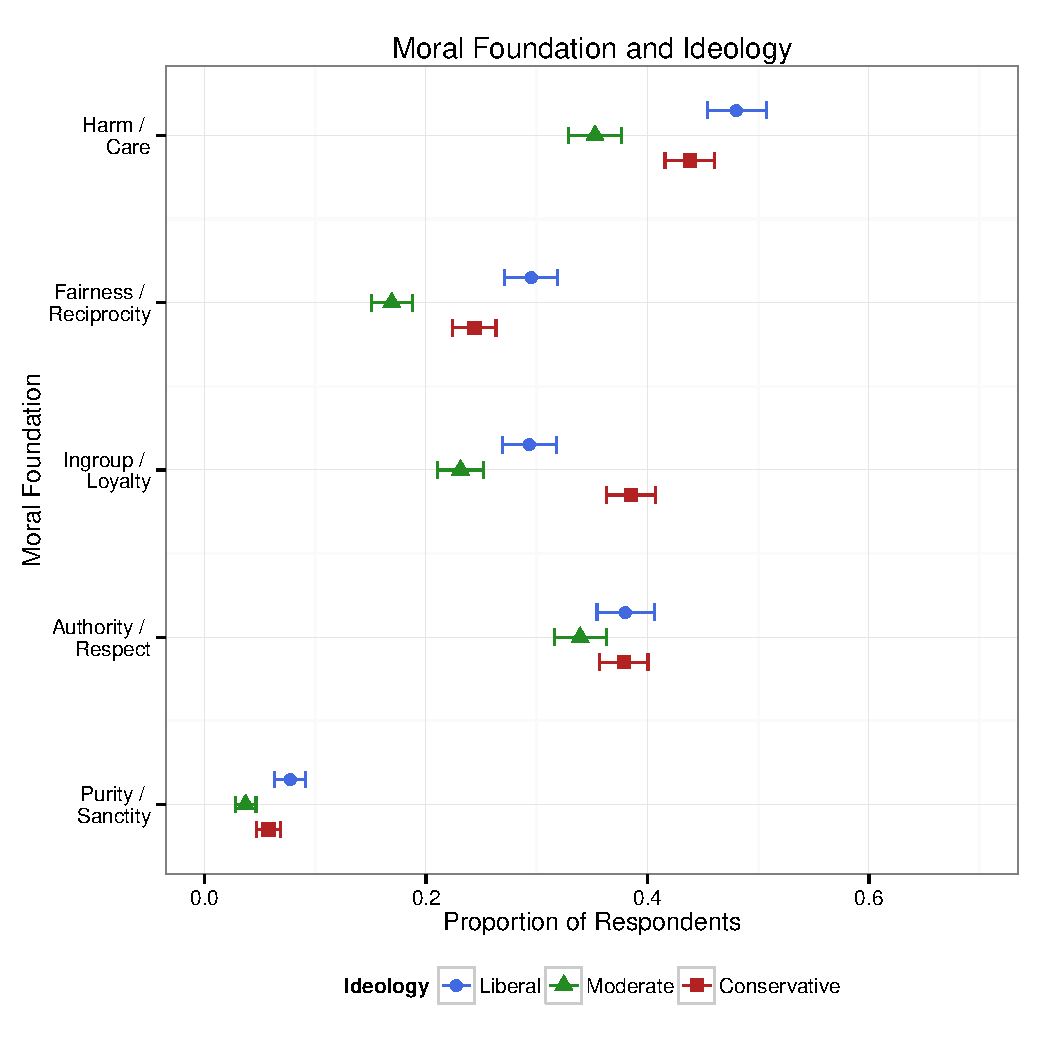
\includegraphics[scale=.4]{../calc/fig/p1_mft_ideol.pdf}
\caption{Moral Foundations and Ideology (all Statements)}\label{fig:mft_ideol}
\end{figure}

The patterns are largely consistent with our theoretical expectations. Liberals were most likely to mention the harm/care foundation. About half of the respondents who identified as liberals mentioned words belonging to this category in their responses. Furthermore, they were more likely than conservatives to mention the fairness/reciprocity foundation. However, it should be noted that fairness/reciprocity was emphasized significantly less than the authority/respect foundation among liberals. Even more surprising is the fact that the proportion of liberal respondents referencing authority/respect is actually larger than the proportion of conservatives. These results, which are inconsistent with previous evidence on moral foundations, as well as the fact that the purity/sanctity foundation was almost never mentioned by any of the respondents suggests that subsequent analyses of survey responses might necessitate a revision of the moral foundation dictionary which was originally developed in the context of sermons. Accordingly, some of the words (e.g. in the case of purity/sanctity) are just too uncommon in the political context. Due to the very rare mentioning of the purity/sanctity dimension, the subsequent analyses will only concentrate on the remaining four moral foundations.

\begin{figure}\centering
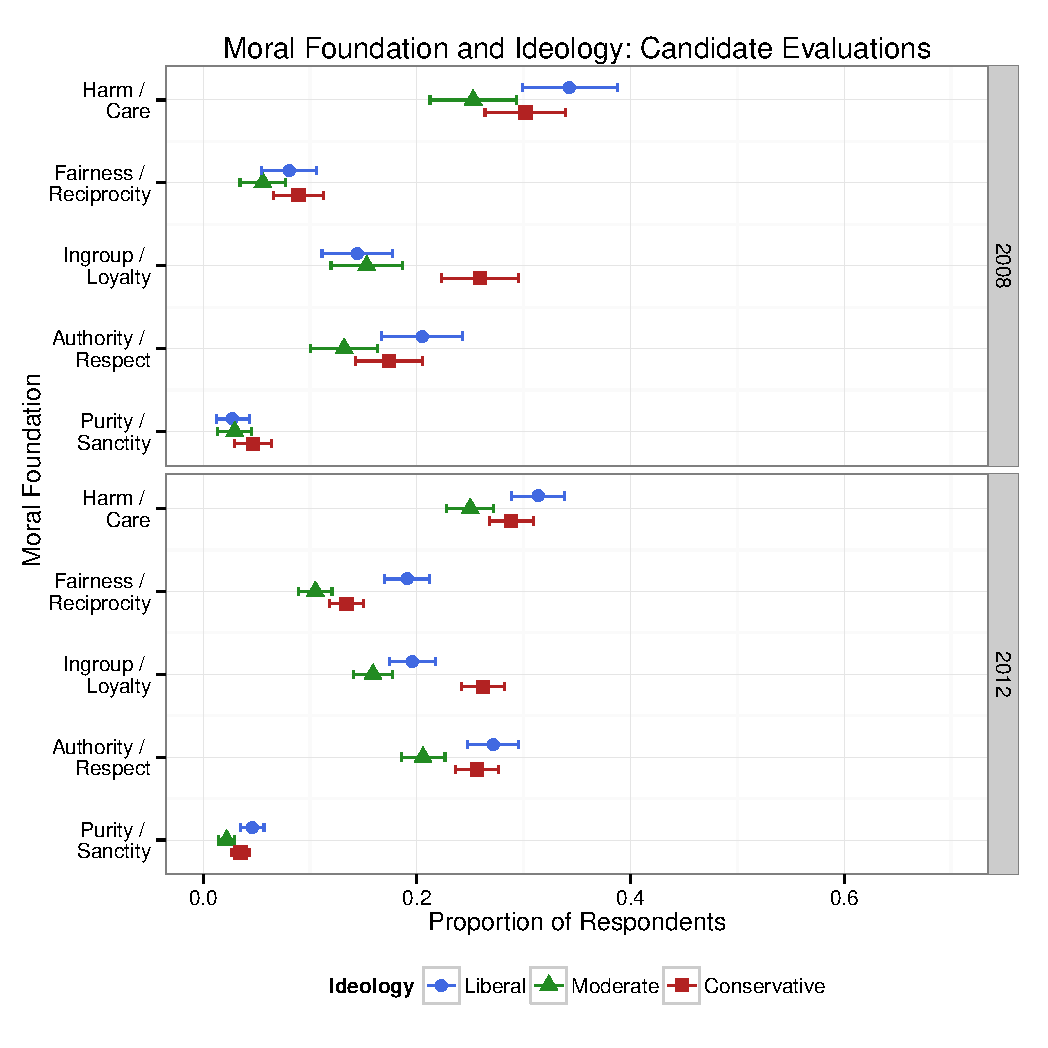
\includegraphics[scale=.4]{../calc/fig/p2_mft_ideol_ca.pdf}
\caption{Moral Foundations and Ideology (Party Evaluations)}\label{fig:mft_ideol_pa}
\end{figure}

\begin{figure}\centering
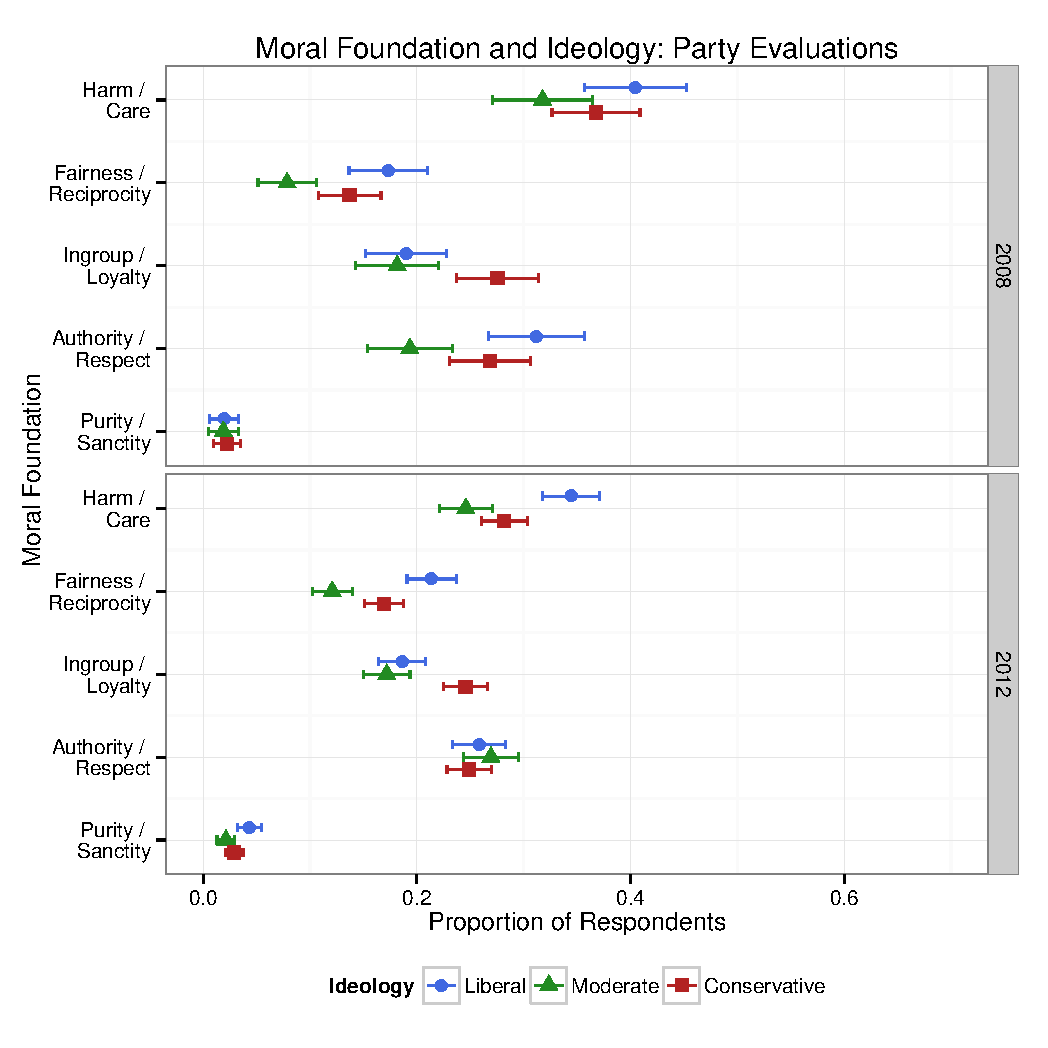
\includegraphics[scale=.4]{../calc/fig/p3_mft_ideol_pa.pdf}
\caption{Moral Foundations and Ideology (Candidate Evaluations)}\label{fig:mft_ideol_ca}
\end{figure}

Instead of looking at the aggregation of all survey items, we can also investigate the patterns in smaller subsets of responses. Figure~\ref{fig:mft_ideol_pa} depicts the same proportions of references to moral foundations combining all open-ended responses related to the Republican and Democratic party. Figure~\ref{fig:mft_ideol_ca}, on the other hand, displays the equivalent results for the responses related to both presidential candidates.

The patterns are similar to the pooled analyses. Conservatives tend to emphasize all moral foundations slightly more equally than liberals. However, disregarding  purity/sanctity, the lowest proportion of conservative respondents mentioned words related to the fairness/reciprocity dimension. These patterns hold irrespective of whether we look at the responses related to presidential candidates or political parties. Overall, these results provide an inconclusive picture on the moral foundations of political reasoning. While some patterns are consistent with our theoretical expectations (e.g. looking at harm/care), the high proportion of liberal respondent mentioning the authority/respect dimension appear to be incoherent with previous empirical accounts. Furthermore, these results are similar if respondents are differentiated by partisanship rather than political ideology (see Appendix B).

Table~\ref{tab:m2_specific} displays the estimates of the logistic regressions predicting the reference to either moral foundation (excluding purity/sanctity). Again, equivalent to the discussion of figure~\ref{fig:mft_ideol}, the responses for each individual was collapsed such that the dependent variables indicate whether any of the responses contained a reference to the moral foundations as identified by the dictionary. Each model includes dummy variables indicating whether the respondents identified as conservative or moderate. Accordingly, the coefficient for conservatives can be directly interpreted as the comparison to the reference category, namely respondents who identified as liberals.


The first column for each moral foundation only looks at the effects of ideology and political interest without taking into account the potential interaction between both variables. Looking at the coefficients for conservatives, we find that the effects are consistent with our first hypothesis for three out of five moral foundations. Conservatives are significantly less likely to mention harm/care and fairness/reciprocity when evaluating political parties and candidates than liberals. Conversely, being conservative increases the likelihood of mentioning words that belong to the category of ingroup/loyalty. However, as already indicated in the previous discussion of the descriptive patterns, liberals appear to be significantly more likely to reference the moral foundation of authority/respect when evaluating political actors. This result is inconsistent with previous evidence for the prevalence of of authority/respect among conservatives. It is worth noting, however, that once partisanship is included in the analyses, the conservatives have a significantly positive effect for this moral foundation as well (see Appendix C).

In order to assess whether these effects are also substantively important, I calculated the differences in predicted probabilities to refer to either of the moral foundations between liberals and conservatives based on the models discussed in table~\ref{tab:m2_specific} (not including the interaction effects). The results are displayed in figure~\ref{fig:models}, along with 95\% confidence intervals. All other variables were held constant at their mean (for continuous variables) or their median (for dichotomous variables). Positive values indicate a higher probability to mention the respective moral foundation in a response among respondents who identified as liberals while negative values indicate a higher probability among conservatives. Accordingly, the probability to mention a word connected to the harm/care foundation is about 7.5 percentage points higher among liberals than conservatives. The effect is slightly stronger for the fairness/reciprocity dimension. Substantively, the ideological difference in the ingroup/loyalty foundation appears to be smallest. The probability to refer to the moral foundation decreases by less than 5 percentage points among liberals as compared to conservatives.

\begin{figure}\centering
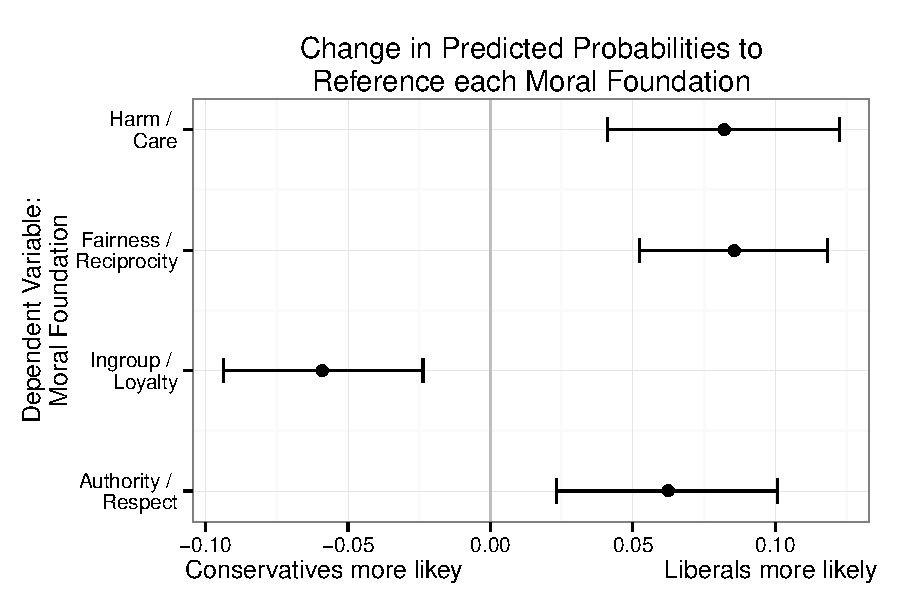
\includegraphics[scale=.4]{../calc/fig/m1_mft.pdf}
\caption{Difference in Predicted Probabilities to Reference each Moral Foundation between Liberals and Conservatives}\label{fig:m1_mft}
\end{figure}

Political interest itself has a significant positive effect for any of the moral foundations considered in the analyses. Irrespective of the specific dimension, individuals with higher political interest are more likely to refer to moral values when talking about their political preferences. This result indicates that political sophistication and expertise in general increases the extent to which respondents take into account moral considerations in the political context, without necessarily differentiating between the respective dimensions. A similar effect can be observed for education as well. One possible explanation for these homogeneous effects could be the fact that the analyses did not control for individual response lengths. Accordingly, since it could be expected that educated and politically interested individuals provide more detailed answers to each of the questions, the likelihood of mentioning any of the words included in the moral foundations dictionary increases by `pure chance'. Subsequent analyses should include a word count for each individual as an additional covariate in order to account for these differences. Another interesting result is the fact that religiosity (measured by church attendance) does not appear to have a significant effect on the likelihood to mention any of the moral foundations except ingroup/loyalty.

\begin{figure}\centering
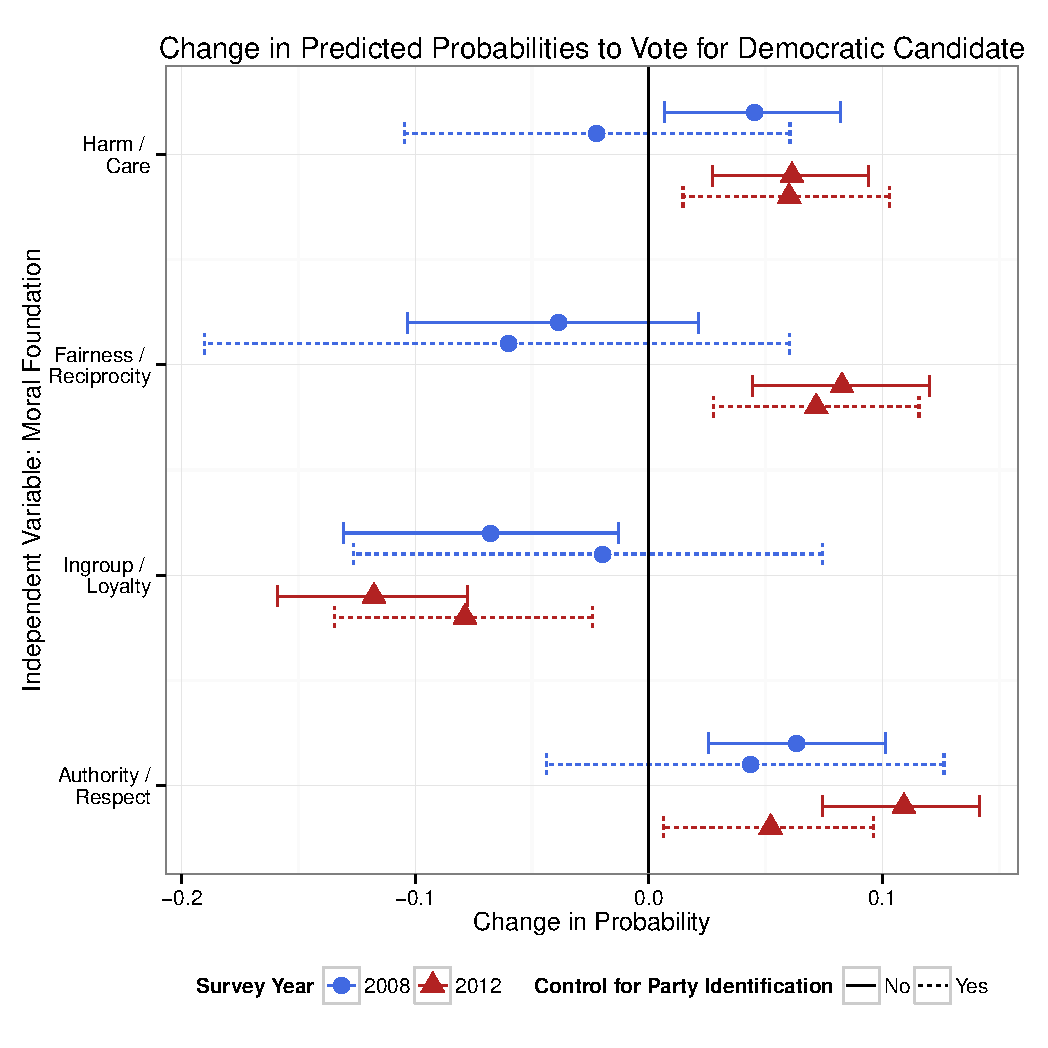
\includegraphics[scale=.4]{../calc/fig/m2_vote.pdf}
\caption{Change in Predicted Probabilities to Vote for Democratic Candidate Depending on References to Specific Moral Foundations}\label{fig:m2_vote}
\end{figure}

\begin{figure}\centering
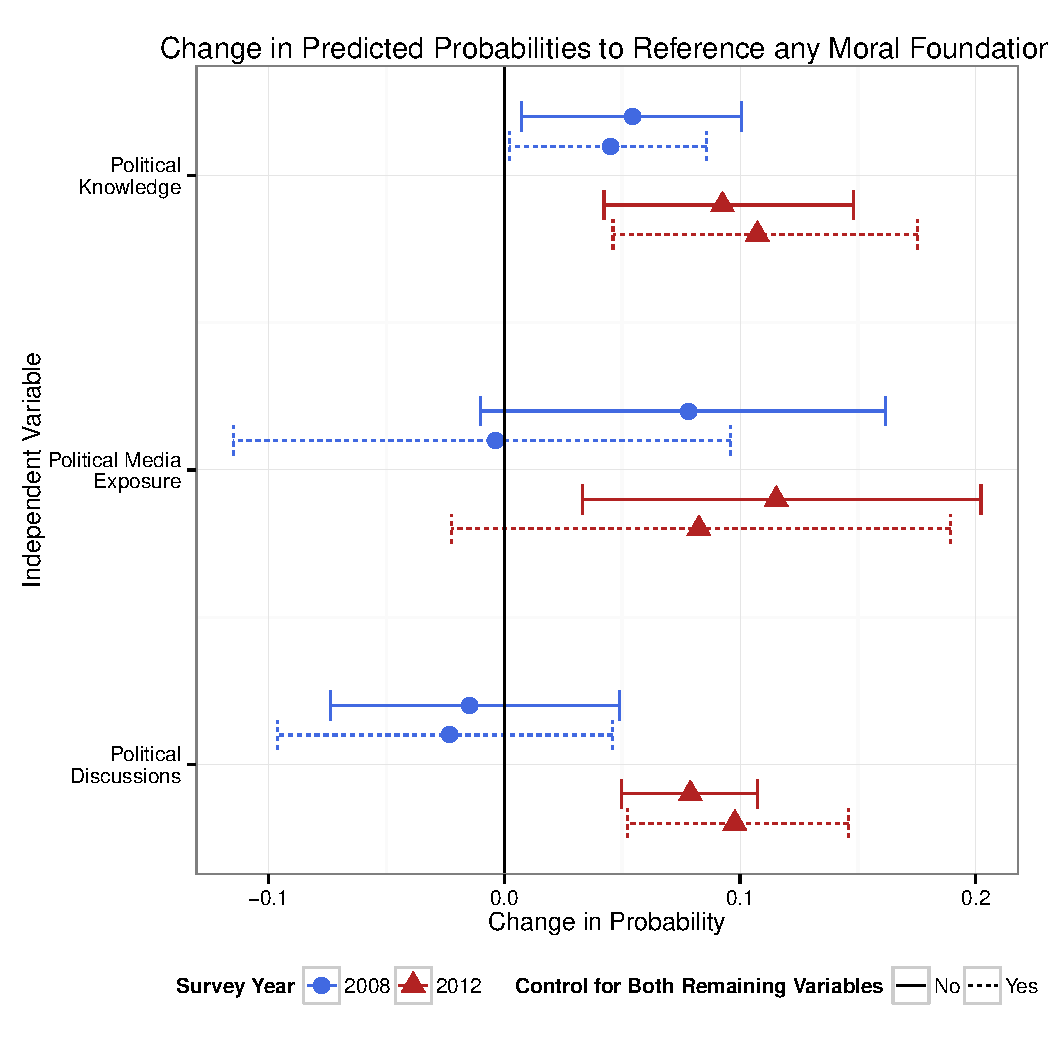
\includegraphics[scale=.4]{../calc/fig/m3_learn.pdf}
\caption{Change in Predicted Probabilities to Reference any of the Moral Foundations Depending on Political Knowledge, Media Exposure, and Frequency of Political Discussions}\label{fig:m3_learn}
\end{figure}

The models presented in the right column for each of the moral foundations in table~\ref{tab:m2_specific} additionally include interaction terms between political interest and ideology. It can be directly observed that the interactions are insignificant for each of the moral foundations included in the analyses. As such, political interest does not moderate the ideological differences in the emphasis on specific moral foundations. Furthermore, comparing the Akaike information criterion between models including and excluding the interaction effects suggests that the inclusion does not increase the fit of any of the models. This result provides no support for the second hypothesis. Accordingly, the empirical evidence appears to be more consistent with the notion that moral foundations provide a universal framework that shapes how individual political reasoning rather than a rhetoric device that is employed among highly sophisticated individuals in order to support their political views.

\begin{figure}\centering
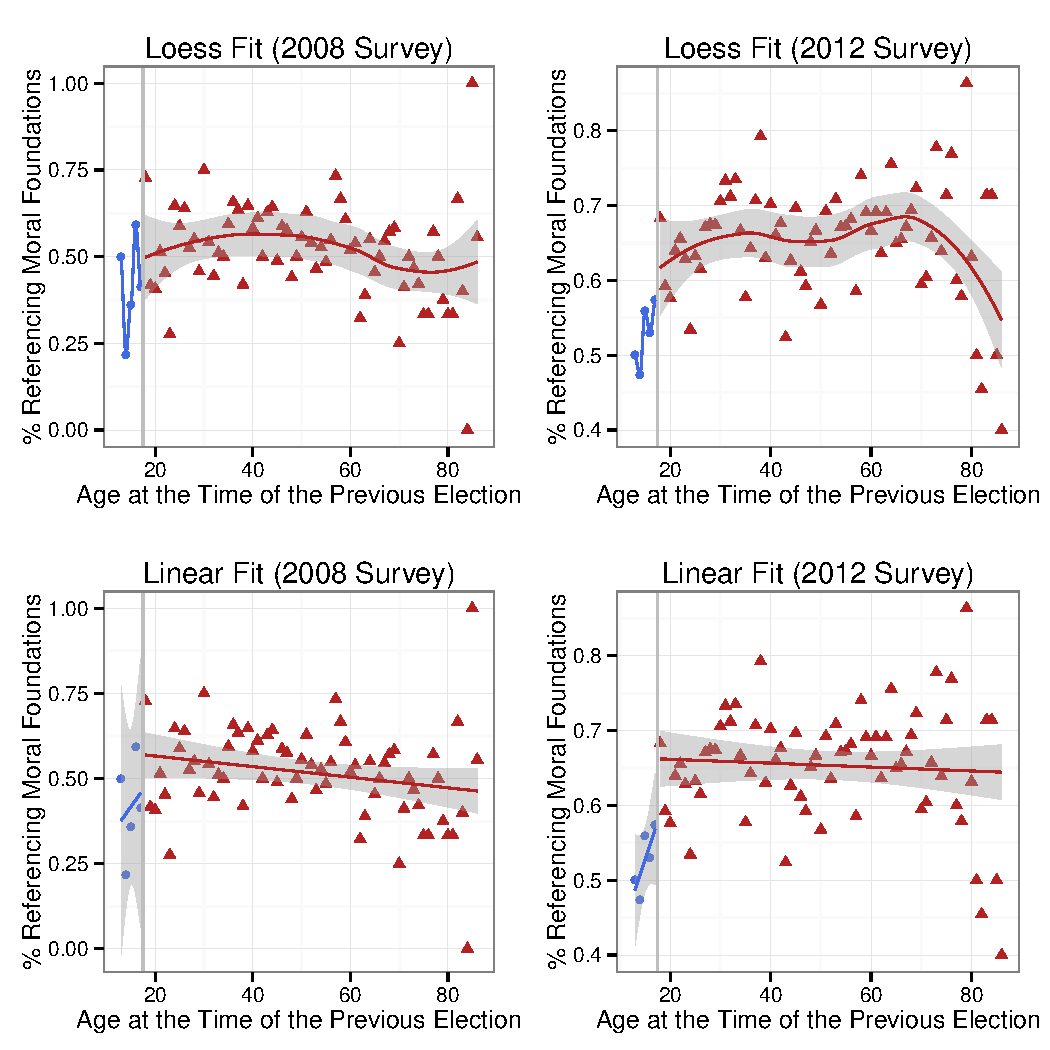
\includegraphics[scale=.8]{../calc/fig/rd1_overview.pdf}
\caption{Visualization of Regression Discontinuity. Proportions Based on Aggregation for Each Age Group (by year).}\label{fig:m2_vote}
\end{figure}

% latex table generated in R 3.1.3 by xtable 1.7-4 package
% Sun Apr 12 13:51:23 2015
\begin{table}[ht]
\centering
\begin{tabular}{lrrrrrrr}
  \hline
 & Bandwidth & Obs. & Est. & SE & Pr($>$$|$z$|$) & CI (low) & CI (high) \\ 
  \hline
LATE & 2.5302 & 166 & 0.5277 & 0.2016 & 0.0088 & 0.1327 & 0.9227 \\ 
  Half-BW & 1.2651 & 51 & 0.3135 & 0.1345 & 0.0198 & 0.0499 & 0.5771 \\ 
  Double-BW & 5.0604 & 268 & 0.1204 & 0.1333 & 0.3666 & -0.1409 & 0.3817 \\ 
   \hline
\end{tabular}
\caption{Regression Discontinuity Estimates Based on Age (2008)} 
\label{tab:rd2008y}
\end{table}

% latex table generated in R 3.2.2 by xtable 1.7-4 package
% Wed Sep 16 10:57:50 2015
\begin{table}[ht]
\centering
\begin{tabular}{lrrrrrrr}
  \hline
 & Bandwidth & Obs. & Est. & SE & Pr($>$$|$z$|$) & CI (low) & CI (high) \\ 
  \hline
LATE & 3.0998 & 415 & 0.1051 & 0.1075 & 0.3285 & 0.0960 & 0.8472 \\ 
  Half-BW & 1.5499 & 280 & 0.1123 & 0.1340 & 0.4020 & 0.0324 & 0.5475 \\ 
  Double-BW & 6.1997 & 672 & 0.0493 & 0.0840 & 0.5574 & -0.1696 & 0.3473 \\ 
   \hline
\end{tabular}
\caption{Regression Discontinuity Estimates Based on Age (2012)} 
\label{tab:rd2012y}
\end{table}

% latex table generated in R 3.1.2 by xtable 1.7-4 package
% Mon Dec 15 04:00:25 2014
\begin{table}[ht]
\centering
\begin{tabular}{lrrrrrrr}
  \hline
 & Bandwidth & Obs. & Est. & SE & Pr($>$$|$z$|$) & CI (low) & CI (high) \\ 
  \hline
LATE & 4.8134 & 17 & 0.2086 & 0.4915 & 0.6712 & 0.1327 & 0.9227 \\ 
  Half-BW & 2.4067 & 8 & 0.9167 & 0.7743 & 0.2365 & 0.0499 & 0.5771 \\ 
  Double-BW & 9.6268 & 41 & 0.4598 & 0.3405 & 0.1769 & -0.1409 & 0.3817 \\ 
   \hline
\end{tabular}
\caption{Regression Discontinuity Estimates Based on Month of Birth (2008)} 
\label{tab:rd2008m1}
\end{table}

% latex table generated in R 3.1.2 by xtable 1.7-4 package
% Sun Dec 14 15:16:33 2014
\begin{table}[ht]
\centering
\begin{tabular}{lrrrrrrr}
  \hline
 & Bandwidth & Obs. & Est. & SE & Pr($>$$|$z$|$) & CI (low) & CI (high) \\ 
  \hline
LATE & 20.0000 & 90 & 0.5646 & 0.2317 & 0.0148 & 0.1327 & 0.9227 \\ 
  Half-BW & 10.0000 & 41 & 0.4745 & 0.3350 & 0.1566 & 0.0499 & 0.5771 \\ 
  Double-BW & 40.0000 & 175 & 0.3802 & 0.1609 & 0.0181 & -0.1409 & 0.3817 \\ 
   \hline
\end{tabular}
\caption{Regression Discontinuity Estimates Based on Month of Birth (2008)} 
\label{tab:rd2008m2}
\end{table}


\section{Limitations}

\section{Conclusion}

The goal of this paper was to investigate to what extent the ideological differences in the emphasis on moral foundations manifests itself in individual reasoning about political actors. It was argued that the analyses of open-ended survey responses can provide important insights beyond previous research because it allows to evaluate in how far citizens make reference to moral considerations in a political context that does not induce an explicit connection to morality. Furthermore, it was argued that the possible moderating effect of political interest on the relationship between ideology and the emphasis on moral foundations allows for further inferences about the role of moral foundations as an underlying factor determining political beliefs or merely a rhetoric device.

The empirical evidence discussed in this paper is mostly consistent with previous results on moral foundations and ideology. The first hypothesis, which predicted systematic patterns in the emphasis on moral considerations among liberals and conservatives was supported for three out of four foundations included in the analyses. On the other hand, the analyses presented in this paper provided no support for the second hypothesis. Political interest did not appear to moderate the relationship between ideology and moral foundations, which in turn suggests that moral values are indeed a universal underlying factor differentiating liberals and conservatives.

However, the fact that purity/sanctity was almost never mentioned as well as the inconsistent effect of ideology on the authority/respect dimension could be attributed to the fact that the moral foundations dictionary was originally conceptualized for the analyses of sermons rather than in the context of day-to-day politics. Accordingly, subsequent analyses should revise the dictionary in order to make it more applicable for the analyses of survey responses. Furthermore, it should be noted that the modelling strategy based on multiple logistic regressions assumes independence between the different response categories. This assumptions does not seem to be plausible since the reference to a specific moral foundation might well affect in how far individuals mention other considerations. While a multinomial logit / conditional logit framework is also not feasible due to the fact that individuals can fall in several categories, other model approaches for non-exclusive multinomial choices might allow to improve the empirical analyses \citep[see for example][]{gilbert2007models}.

An alternative approach to the analysis of open-ended survey responses could be the implementation of structural topic models as described by \citet{roberts2014structural}: Instead of using explicit word lists to identify moral reasoning, it would possible to identify specific topics in open-ended responses that are consistent with the moral foundations described by \citet{haidt2008moral} \citep[see also][]{lin2008joint}.

Notwithstanding these reservations and the resulting tentativeness of the empirical results presented thus far, the analyses of open-ended survey responses can provide important and valuable insights in the context of moral foundations and the individual underpinnings of political ideology. As such, there are numerous avenues for future research. For example, it would be interesting to investigate the degree to which contextual factors such as campaign exposure and social networks affect political (and moral) reasoning among individuals. Furthermore, it could be analyzed whether the reference to specific moral foundations differs between survey questions: Do individuals differ in terms of their moral considerations if they describe in-party or out-party candidates? Does the evaluations of parties and candidate elicit different considerations? Furthermore, are there sources of heterogeneity in moral foundations among liberals and conservatives? Utilizing available responses to open-ended survey questions provides a useful and still largely neglected data source to investigate these and other important research questions from novel perspectives.


\clearpage\flushleft\footnotesize
\appendices
\section{Moral Foundations Dictionary}
\renewcommand\thefigure{\thesection.\arabic{figure}}
\renewcommand\thetable{\thesection.\arabic{table}}
\setcounter{figure}{0}
\setcounter{table}{0}

\textit{Sources:}\\
\citet{graham2009liberals}, as well as \url{http://www.moralfoundations.org/}
\vspace{.5cm}

\textit{Note:}\\
Words with (*) indicate that the word stem rather than the exact word was matched in the open-ended survey responses.
\vspace{.5cm}

\textbf{Harm:}\\
safe*, peace*, compassion*, empath*, sympath*, care, caring, protect*, shield, shelter, amity, secur*, benefit*, defen*, guard*, preserve, harm*, suffer*, war, wars, warl*, warring, fight*, violen*, hurt*, kill, kills, killer*, killed, killing, endanger*, cruel*, brutal*, abuse*, damag*, ruin*, ravage, detriment*, crush*, attack*, annihilate*, destroy, stomp, abandon*, spurn, impair, exploit, exploits, exploited, exploiting, wound*
\vspace{.5cm}

\textbf{Fairness:}\\
fair, fairly, fairness, fair*, fairmind*, fairplay, equal*, justice, justness, justifi*, reciproc*, impartial*, egalitar*, rights, equity, evenness, equivalent, unbias*, tolerant, equable, balance*, homologous, unprejudice*, reasonable, constant, honest*, unfair*, unequal*, bias*, unjust*, injust*, bigot*, discriminat*, disproportion*, inequitable, prejud*, dishonest, unscrupulous, dissociate, preference, favoritism, segregat*, exclusion, exclud*
\vspace{.5cm}

\textbf{Ingroup:}\\
together, nation*, homeland*, family, families, familial, group, loyal*, patriot*, communal, commune*, communit*, communis*, comrad*, cadre, collectiv*, joint, unison, unite*, fellow*, guild, solidarity, devot*, member, cliqu*, cohort, ally, insider, foreign*, enem*, betray*, treason*, traitor*, treacher*, disloyal*, individual*, apostasy, apostate, deserted, deserter*, deserting, deceiv*, jilt*, imposter, miscreant, spy, sequester, renegade, terroris*, immigra*
\vspace{.5cm}

\textbf{Authority:}\\
obey*, obedien*, duty, law, lawful*, legal*, duti*, honor*, respect, respectful*, respected, respects, order*, father*, mother, motherl*, mothering, mothers, tradition*, hierarch*, authorit*, permit, permission, status*, rank*, leader*, class, bourgeoisie, caste*, position, complian*, command, supremacy, control, submi*, allegian*, serve, abide, defere*, defer, revere*, venerat*, comply, defian*, rebel*, dissent*, subver*, disrespect*, disobe*, sediti*, agitat*, insubordinat*, illegal*, lawless*, insurgent, mutinous, defy*, dissident, unfaithful, alienate, defector, heretic*, nonconformist, oppose, protest, refuse, denounce, remonstrate, riot*, obstruct
\vspace{.5cm}

\textbf{Purity:}\\
piety, pious, purity, pure*, clean*, steril*, sacred*, chast*, holy, holiness, saint*, wholesome*, celiba*, abstention, virgin, virgins, virginity, virginal, austerity, integrity, modesty, abstinen*, abstemiousness, upright, limpid, unadulterated, maiden, virtuous, refined, intemperate, decen*, immaculate, innocent, pristine, humble, disgust*, deprav*, disease*, unclean*, contagio*, indecen*, sin, sinful*, sinner*, sins, sinned, sinning, slut*, whore, dirt*, impiety, impious, profan*, gross, repuls*, sick*, promiscu*, lewd*, adulter*, debauche*, defile*, tramp, prostitut*, unchaste, wanton, profligate, filth*, trashy, obscen*, lax, taint*, stain*, tarnish*, debase*, desecrat*, wicked*, blemish, exploitat*, pervert, wretched*


\clearpage
\section{Additional Tables and Figures - Overview}
\renewcommand\thefigure{\thesection.\arabic{figure}}
\renewcommand\thetable{\thesection.\arabic{table}}
\setcounter{figure}{0}
\setcounter{table}{0}

% latex table generated in R 3.2.2 by xtable 1.7-4 package
% Wed Sep 16 10:56:58 2015
\begin{table}[ht]
\centering
\begin{tabular}{lcc}
  \hline
 & N & Percent \\ 
  \hline
Spanish Interview (2008) & 94 & 4.05 \\ 
  Spanish Interview (2012) & 228 & 3.86 \\ 
  No Responses (Overall, 2008) & 158 & 7.09 \\ 
  No Responses (Overall, 2012) & 392 & 6.89 \\ 
  No Responses (Candidate Evaluations, 2008) & 328 & 14.13 \\ 
  No Responses (Candidate Evaluations, 2012) & 761 & 12.87 \\ 
  No Responses (Party Evaluations, 2008) & 584 & 25.15 \\ 
  No Responses (Party Evaluations, 2012) & 1503 & 25.41 \\ 
   \hline
\end{tabular}
\caption{Overview - Missing Open-Ended Responses} 
\label{tab:a1_mis}
\end{table}


\begin{figure}[ht]\centering
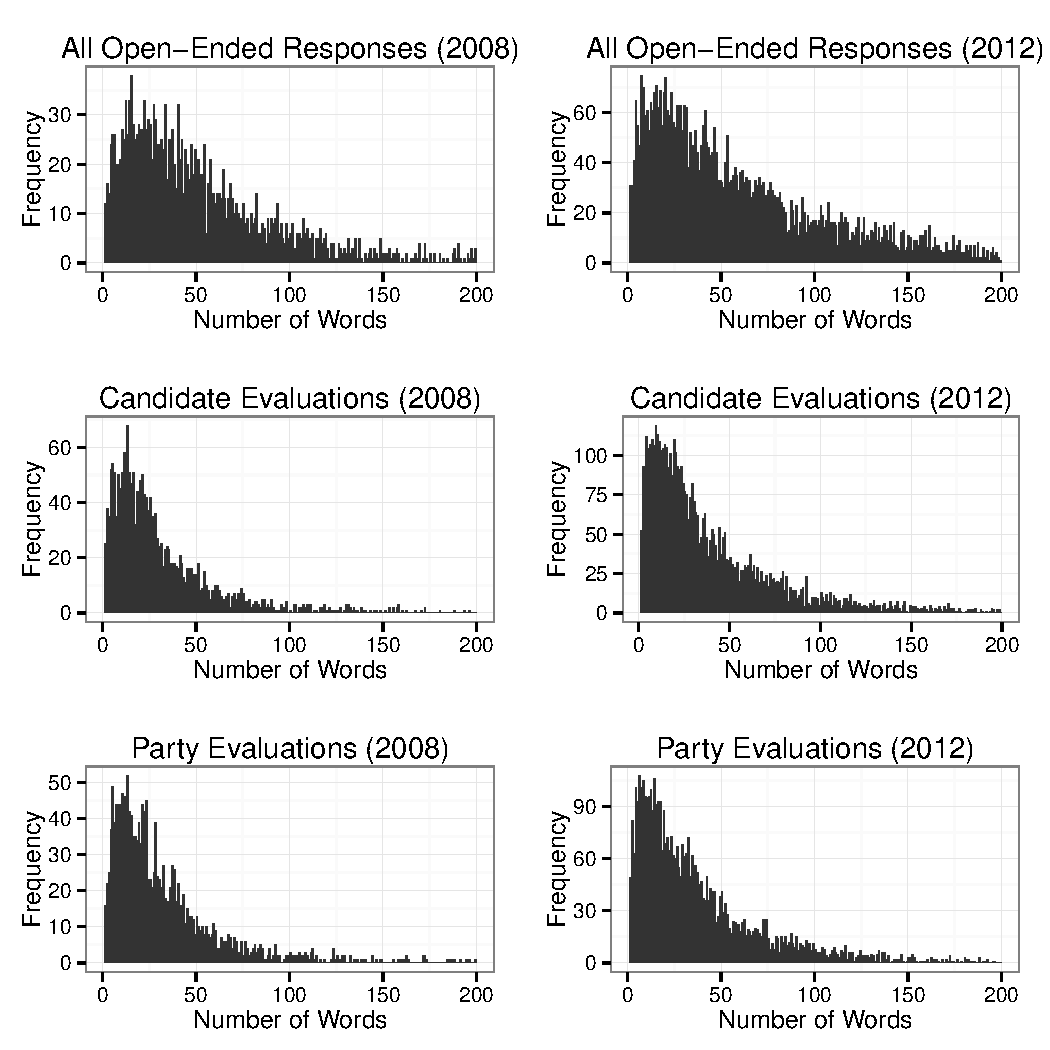
\includegraphics[scale=.8]{../calc/fig/a0_num.pdf}
\caption{Distribution of Numbers of Words in Open-Ended Responses}\label{fig:a0_num}
\end{figure}

\begin{figure}[ht]\centering
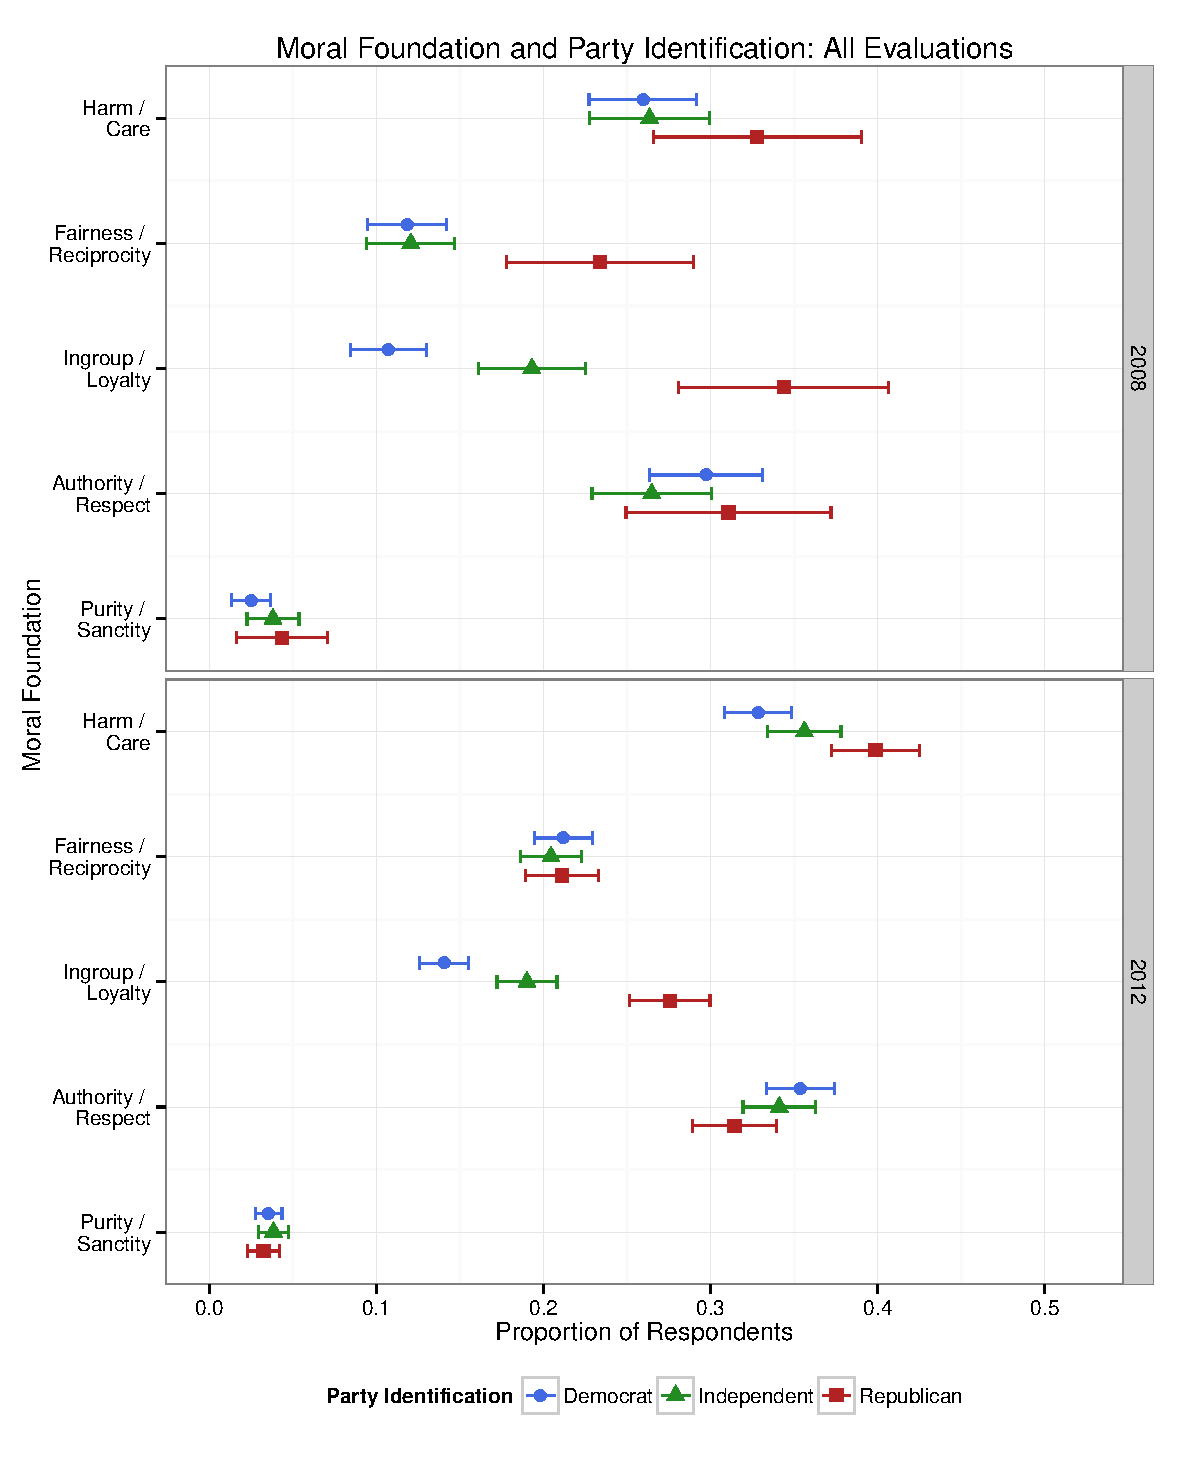
\includegraphics[scale=.4]{../calc/fig/a1_mft_pid.pdf}
\caption{Moral Foundations and Partisanship (all Statements)}\label{fig:a1_mft_pid}
\end{figure}

\begin{figure}[ht]\centering
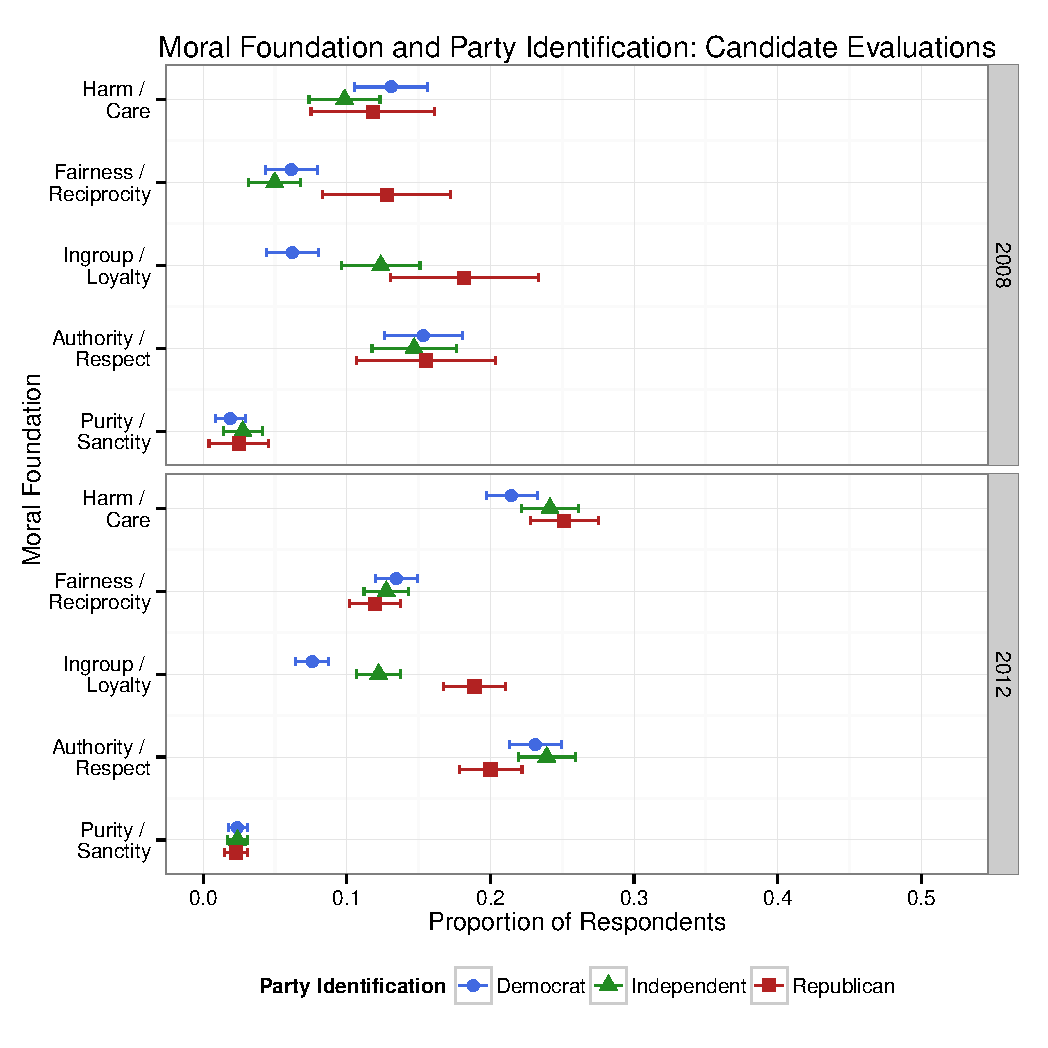
\includegraphics[scale=.4]{../calc/fig/a2_mft_pid_ca.pdf}
\caption{Moral Foundations and Partisanship (Candidate Evaluations)}\label{fig:a2_mft_pid_ca}
\end{figure}

\begin{figure}[ht]\centering
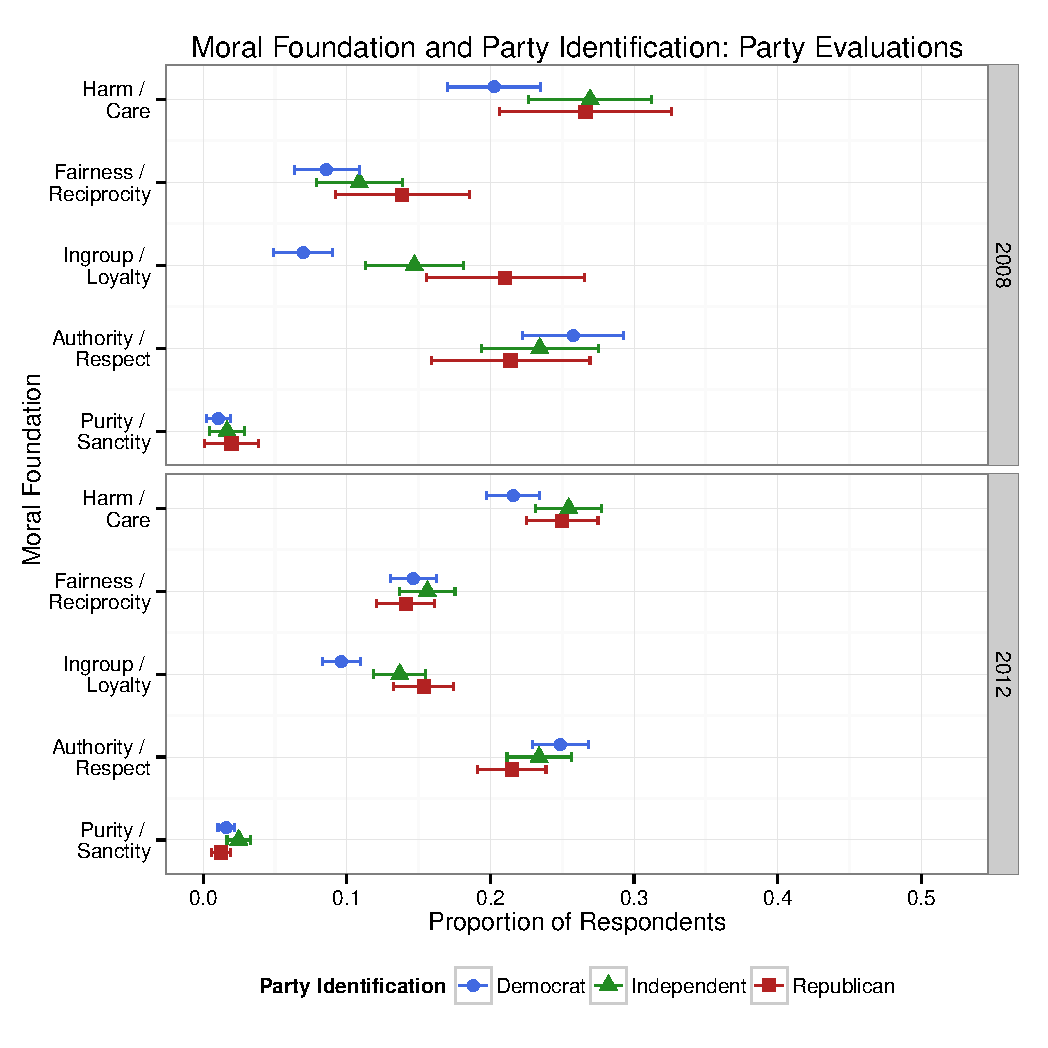
\includegraphics[scale=.4]{../calc/fig/a3_mft_pid_pa.pdf}
\caption{Moral Foundations and Partisanship (Party Evaluations)}\label{fig:a3_mft_pid_pa}
\end{figure}


\clearpage
\section{Tables of Logit Model Estimates}
\renewcommand\thefigure{\thesection.\arabic{figure}}
\renewcommand\thetable{\thesection.\arabic{table}}
\setcounter{figure}{0}
\setcounter{table}{0}


% Table created by stargazer v.5.2 by Marek Hlavac, Harvard University. E-mail: hlavac at fas.harvard.edu
% Date and time: Wed, Sep 16, 2015 - 10:57:06 AM
% Requires LaTeX packages: dcolumn 
\begin{table}[ht] \centering 
  \caption{Logit Models Predicting References to four Moral Foundations using Ideology} 
  \label{tab:m1_mft} 
\tiny 
\begin{tabular}{@{\extracolsep{-15pt}}lD{.}{.}{-3} D{.}{.}{-3} D{.}{.}{-3} D{.}{.}{-3} D{.}{.}{-3} D{.}{.}{-3} D{.}{.}{-3} D{.}{.}{-3} } 
\\[-1.8ex]\hline 
\hline \\[-1.8ex] 
 & \multicolumn{8}{c}{\textit{Dependent variable:}} \\ 
\cline{2-9} 
\\[-1.8ex] & \multicolumn{2}{c}{Harm / Care} & \multicolumn{2}{c}{Fairness / Reciprocity} & \multicolumn{2}{c}{Ingroup / Loyalty} & \multicolumn{2}{c}{Authority / Respect} \\ 
 & \multicolumn{1}{c}{2008} & \multicolumn{1}{c}{2012} & \multicolumn{1}{c}{2008} & \multicolumn{1}{c}{2012} & \multicolumn{1}{c}{2008} & \multicolumn{1}{c}{2012} & \multicolumn{1}{c}{2008} & \multicolumn{1}{c}{2012} \\ 
\hline \\[-1.8ex] 
 Conservative & -0.105 & -0.327^{***} & -0.005 & -0.440^{***} & 0.288 & 0.407^{***} & -0.342^{**} & -0.308^{***} \\ 
  & (0.160) & (0.084) & (0.198) & (0.093) & (0.192) & (0.104) & (0.153) & (0.085) \\ 
  Moderate & -0.144 & -0.383^{***} & -0.280 & -0.480^{***} & 0.158 & 0.133 & -0.442^{***} & -0.129 \\ 
  & (0.165) & (0.085) & (0.217) & (0.096) & (0.202) & (0.110) & (0.159) & (0.085) \\ 
  Church Attendance & -0.025 & -0.014 & -0.015 & 0.002 & 0.052 & 0.074^{***} & 0.064^{*} & -0.026 \\ 
  & (0.039) & (0.020) & (0.048) & (0.022) & (0.044) & (0.023) & (0.037) & (0.020) \\ 
  Education (College Degree) & 0.318^{**} & 0.032 & 0.306^{*} & 0.315^{***} & 0.458^{***} & 0.138^{*} & 0.321^{**} & 0.235^{***} \\ 
  & (0.140) & (0.070) & (0.182) & (0.077) & (0.171) & (0.083) & (0.134) & (0.070) \\ 
  Age & -0.017^{***} & -0.004^{**} & 0.010^{**} & 0.003 & 0.001 & 0.002 & -0.004 & 0.008^{***} \\ 
  & (0.004) & (0.002) & (0.005) & (0.002) & (0.005) & (0.002) & (0.004) & (0.002) \\ 
  Sex (Female) & 0.074 & 0.274^{***} & 0.154 & 0.133^{*} & -0.085 & -0.007 & -0.182 & -0.069 \\ 
  & (0.129) & (0.067) & (0.164) & (0.076) & (0.152) & (0.081) & (0.124) & (0.067) \\ 
  Race (African American) & -0.044 & -0.028 & -0.102 & -0.139 & 0.235 & 0.012 & -0.071 & 0.417^{***} \\ 
  & (0.166) & (0.092) & (0.219) & (0.108) & (0.191) & (0.114) & (0.160) & (0.091) \\ 
  Number of Words & 0.013^{***} & 0.011^{***} & 0.008^{***} & 0.008^{***} & 0.011^{***} & 0.011^{***} & 0.010^{***} & 0.012^{***} \\ 
  & (0.001) & (0.001) & (0.001) & (0.0005) & (0.001) & (0.001) & (0.001) & (0.001) \\ 
  Constant & -1.193^{***} & -1.108^{***} & -3.164^{***} & -1.935^{***} & -3.062^{***} & -2.839^{***} & -1.362^{***} & -1.811^{***} \\ 
  & (0.249) & (0.126) & (0.335) & (0.144) & (0.315) & (0.163) & (0.241) & (0.132) \\ 
 \hline \\[-1.8ex] 
Observations & \multicolumn{1}{c}{1,468} & \multicolumn{1}{c}{4,691} & \multicolumn{1}{c}{1,468} & \multicolumn{1}{c}{4,691} & \multicolumn{1}{c}{1,468} & \multicolumn{1}{c}{4,691} & \multicolumn{1}{c}{1,468} & \multicolumn{1}{c}{4,691} \\ 
Log Likelihood & \multicolumn{1}{c}{-754.236} & \multicolumn{1}{c}{-2,718.587} & \multicolumn{1}{c}{-528.080} & \multicolumn{1}{c}{-2,251.633} & \multicolumn{1}{c}{-586.828} & \multicolumn{1}{c}{-2,015.282} & \multicolumn{1}{c}{-802.048} & \multicolumn{1}{c}{-2,684.276} \\ 
Akaike Inf. Crit. & \multicolumn{1}{c}{1,526.472} & \multicolumn{1}{c}{5,455.174} & \multicolumn{1}{c}{1,074.159} & \multicolumn{1}{c}{4,521.265} & \multicolumn{1}{c}{1,191.656} & \multicolumn{1}{c}{4,048.565} & \multicolumn{1}{c}{1,622.097} & \multicolumn{1}{c}{5,386.553} \\ 
\hline 
\hline \\[-1.8ex] 
\textit{Note:}  & \multicolumn{8}{r}{$^{*}$p$<$0.1; $^{**}$p$<$0.05; $^{***}$p$<$0.01} \\ 
\end{tabular} 
\end{table} 



% Table created by stargazer v.5.2 by Marek Hlavac, Harvard University. E-mail: hlavac at fas.harvard.edu
% Date and time: Tue, Nov 10, 2015 - 12:11:17 PM
% Requires LaTeX packages: dcolumn 
\begin{table}[ht] \centering 
  \caption{Logit Models Predicting Democratic Vote Choice Based on Moral Foundations} 
  \label{tab:m2_vote} 
\tiny 
\begin{tabular}{@{\extracolsep{-15pt}}lD{.}{.}{-3} D{.}{.}{-3} D{.}{.}{-3} D{.}{.}{-3} } 
\\[-1.8ex]\hline 
\hline \\[-1.8ex] 
 & \multicolumn{4}{c}{\textit{Dependent variable:}} \\ 
\cline{2-5} 
\\[-1.8ex] & \multicolumn{4}{c}{Vote for Democratic Presidential Candidate} \\ 
 & \multicolumn{2}{c}{2008} & \multicolumn{2}{c}{2012} \\ 
\\[-1.8ex] & \multicolumn{1}{c}{(1)} & \multicolumn{1}{c}{(2)} & \multicolumn{1}{c}{(3)} & \multicolumn{1}{c}{(4)}\\ 
\hline \\[-1.8ex] 
 Harm / Care & 0.292^{**} & -0.099 & 0.270^{***} & 0.286^{***} \\ 
  & (0.122) & (0.183) & (0.079) & (0.111) \\ 
  Fairness / Reciprocity & -0.207 & -0.245 & 0.376^{***} & 0.344^{***} \\ 
  & (0.167) & (0.273) & (0.090) & (0.124) \\ 
  Ingroup / Loyalty & -0.348^{**} & -0.087 & -0.481^{***} & -0.341^{***} \\ 
  & (0.140) & (0.214) & (0.086) & (0.118) \\ 
  Authority / Respect & 0.408^{***} & 0.209 & 0.507^{***} & 0.245^{**} \\ 
  & (0.132) & (0.200) & (0.081) & (0.111) \\ 
  Party Identification (Democrat) &  & 2.888^{***} &  & 2.592^{***} \\ 
  &  & (0.183) &  & (0.131) \\ 
  Party Identification (Republican) &  & -2.260^{***} &  & -2.560^{***} \\ 
  &  & (0.411) &  & (0.143) \\ 
  Church Attendance & -0.226^{***} & -0.099^{*} & -0.311^{***} & -0.274^{***} \\ 
  & (0.033) & (0.051) & (0.022) & (0.030) \\ 
  Education (College Degree) & -0.362^{***} & -0.343^{*} & 0.077 & 0.213^{**} \\ 
  & (0.121) & (0.177) & (0.079) & (0.108) \\ 
  Age & -0.017^{***} & -0.030^{***} & -0.014^{***} & -0.022^{***} \\ 
  & (0.003) & (0.005) & (0.002) & (0.003) \\ 
  Sex (Female) & 0.388^{***} & 0.101 & 0.365^{***} & 0.306^{***} \\ 
  & (0.117) & (0.172) & (0.075) & (0.103) \\ 
  Race (African American) & 4.330^{***} & 3.693^{***} & 3.974^{***} & 3.056^{***} \\ 
  & (0.390) & (0.468) & (0.229) & (0.256) \\ 
  Constant & 1.269^{***} & 0.592^{**} & 0.743^{***} & 1.007^{***} \\ 
  & (0.207) & (0.291) & (0.136) & (0.190) \\ 
 \hline \\[-1.8ex] 
Observations & \multicolumn{1}{c}{1,822} & \multicolumn{1}{c}{1,313} & \multicolumn{1}{c}{3,973} & \multicolumn{1}{c}{3,963} \\ 
Log Likelihood & \multicolumn{1}{c}{-886.197} & \multicolumn{1}{c}{-453.056} & \multicolumn{1}{c}{-2,096.122} & \multicolumn{1}{c}{-1,237.334} \\ 
Akaike Inf. Crit. & \multicolumn{1}{c}{1,792.393} & \multicolumn{1}{c}{930.112} & \multicolumn{1}{c}{4,212.244} & \multicolumn{1}{c}{2,498.669} \\ 
\hline 
\hline \\[-1.8ex] 
\textit{Note:}  & \multicolumn{4}{r}{$^{*}$p$<$0.1; $^{**}$p$<$0.05; $^{***}$p$<$0.01} \\ 
\end{tabular} 
\end{table} 



% Table created by stargazer v.5.1 by Marek Hlavac, Harvard University. E-mail: hlavac at fas.harvard.edu
% Date and time: Sun, Dec 14, 2014 - 03:16:26 PM
% Requires LaTeX packages: dcolumn 
\begin{table}[ht] \centering 
  \caption{Logit Models Predicting Overall References to Moral Foundations} 
  \label{tab:m3_learn} 
\tiny 
\begin{tabular}{@{\extracolsep{-15pt}}lD{.}{.}{-3} D{.}{.}{-3} D{.}{.}{-3} D{.}{.}{-3} D{.}{.}{-3} D{.}{.}{-3} D{.}{.}{-3} D{.}{.}{-3} } 
\\[-1.8ex]\hline 
\hline \\[-1.8ex] 
 & \multicolumn{8}{c}{\textit{Dependent variable:}} \\ 
\cline{2-9} 
\\[-1.8ex] & \multicolumn{8}{c}{Reference to any Moral Foundation} \\ 
 & \multicolumn{1}{c}{2008} & \multicolumn{1}{c}{2012} & \multicolumn{1}{c}{2008} & \multicolumn{1}{c}{2012} & \multicolumn{1}{c}{2008} & \multicolumn{1}{c}{2012} & \multicolumn{1}{c}{2008} & \multicolumn{1}{c}{2012} \\ 
\\[-1.8ex] & \multicolumn{1}{c}{(1)} & \multicolumn{1}{c}{(2)} & \multicolumn{1}{c}{(3)} & \multicolumn{1}{c}{(4)} & \multicolumn{1}{c}{(5)} & \multicolumn{1}{c}{(6)} & \multicolumn{1}{c}{(7)} & \multicolumn{1}{c}{(8)}\\ 
\hline \\[-1.8ex] 
 Political Knowledge & 0.261^{**} & 0.149^{***} &  &  &  &  & 0.219^{*} & 0.142^{***} \\ 
  & (0.117) & (0.033) &  &  &  &  & (0.125) & (0.035) \\ 
  Political Media Exposure &  &  & 0.027^{***} & 0.019^{***} &  &  & 0.017^{*} & 0.011^{*} \\ 
  &  &  & (0.009) & (0.006) &  &  & (0.010) & (0.006) \\ 
  Political Discussions &  &  &  &  & 0.001 & 0.091^{***} & -0.011 & 0.079^{***} \\ 
  &  &  &  &  & (0.025) & (0.019) & (0.026) & (0.019) \\ 
  Church Attendance & 0.022 & -0.020 & 0.022 & -0.020 & 0.013 & -0.018 & 0.012 & -0.019 \\ 
  & (0.031) & (0.019) & (0.030) & (0.019) & (0.033) & (0.020) & (0.033) & (0.020) \\ 
  Education (College Degree) & 0.379^{***} & 0.185^{**} & 0.442^{***} & 0.239^{***} & 0.480^{***} & 0.282^{***} & 0.402^{***} & 0.183^{**} \\ 
  & (0.114) & (0.077) & (0.106) & (0.075) & (0.116) & (0.077) & (0.121) & (0.081) \\ 
  Age & -0.005 & -0.002 & -0.008^{**} & -0.003 & -0.003 & 0.0002 & -0.004 & -0.003 \\ 
  & (0.003) & (0.002) & (0.003) & (0.002) & (0.003) & (0.002) & (0.004) & (0.002) \\ 
  Sex (Female) & -0.094 & 0.226^{***} & -0.064 & 0.204^{***} & -0.135 & 0.195^{***} & -0.123 & 0.243^{***} \\ 
  & (0.109) & (0.068) & (0.104) & (0.067) & (0.114) & (0.069) & (0.115) & (0.071) \\ 
  Race (African American) & -0.057 & 0.445^{***} & -0.096 & 0.367^{***} & -0.070 & 0.358^{***} & -0.023 & 0.418^{***} \\ 
  & (0.127) & (0.091) & (0.118) & (0.088) & (0.133) & (0.092) & (0.135) & (0.094) \\ 
  Number of Words & 0.029^{***} & 0.025^{***} & 0.029^{***} & 0.026^{***} & 0.028^{***} & 0.025^{***} & 0.027^{***} & 0.025^{***} \\ 
  & (0.002) & (0.001) & (0.002) & (0.001) & (0.002) & (0.001) & (0.002) & (0.001) \\ 
  Constant & -1.411^{***} & -1.319^{***} & -1.481^{***} & -1.067^{***} & -1.274^{***} & -1.066^{***} & -1.484^{***} & -1.464^{***} \\ 
  & (0.201) & (0.143) & (0.195) & (0.122) & (0.209) & (0.124) & (0.227) & (0.152) \\ 
 \hline \\[-1.8ex] 
Observations & \multicolumn{1}{c}{1,845} & \multicolumn{1}{c}{5,147} & \multicolumn{1}{c}{2,031} & \multicolumn{1}{c}{5,177} & \multicolumn{1}{c}{1,648} & \multicolumn{1}{c}{4,842} & \multicolumn{1}{c}{1,646} & \multicolumn{1}{c}{4,807} \\ 
Log Likelihood & \multicolumn{1}{c}{-1,016.596} & \multicolumn{1}{c}{-2,670.308} & \multicolumn{1}{c}{-1,118.869} & \multicolumn{1}{c}{-2,689.725} & \multicolumn{1}{c}{-915.937} & \multicolumn{1}{c}{-2,495.047} & \multicolumn{1}{c}{-912.088} & \multicolumn{1}{c}{-2,467.724} \\ 
Akaike Inf. Crit. & \multicolumn{1}{c}{2,049.192} & \multicolumn{1}{c}{5,356.616} & \multicolumn{1}{c}{2,253.737} & \multicolumn{1}{c}{5,395.450} & \multicolumn{1}{c}{1,847.874} & \multicolumn{1}{c}{5,006.093} & \multicolumn{1}{c}{1,844.175} & \multicolumn{1}{c}{4,955.448} \\ 
\hline 
\hline \\[-1.8ex] 
\textit{Note:}  & \multicolumn{8}{r}{$^{*}$p$<$0.1; $^{**}$p$<$0.05; $^{***}$p$<$0.01} \\ 
\end{tabular} 
\end{table} 


\clearpage
\section{Additional Tables and Figures - Regression Discontinuity}
\renewcommand\thefigure{\thesection.\arabic{figure}}
\renewcommand\thetable{\thesection.\arabic{table}}
\setcounter{figure}{0}
\setcounter{table}{0}

\begin{figure}[ht]\centering
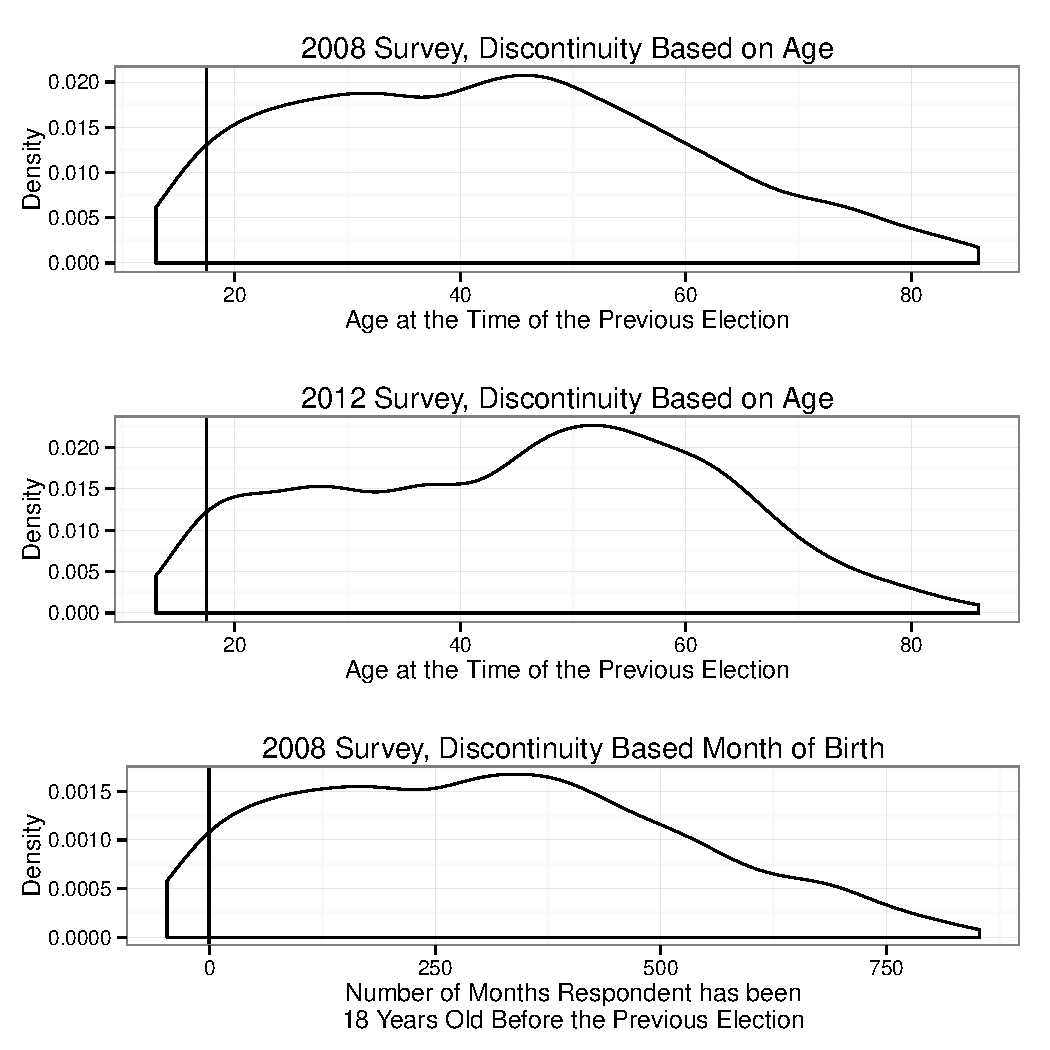
\includegraphics[scale=.5]{../calc/fig/rd2_density.pdf}
\caption{Density of Running Variable (Age / Months)}\label{fig:rd2_density}
\end{figure}

\clearpage
\subsection{Placebo Tests}
% latex table generated in R 3.2.2 by xtable 1.7-4 package
% Tue Sep 15 18:25:32 2015
\begin{table}[ht]
\centering
\begin{tabular}{lrrrrrrr}
  \hline
 & Bandwidth & Obs. & Est. & SE & Pr($>$$|$z$|$) & CI (low) & CI (high) \\ 
  \hline
LATE & 1.8657 & 133 & -0.0271 & 0.1853 & 0.8838 & -0.3902 & 0.3360 \\ 
  Half-BW & 0.9329 & 77 & -0.0619 & 0.1157 & 0.5926 & -0.2886 & 0.1648 \\ 
  Double-BW & 3.7315 & 259 & -0.1248 & 0.1358 & 0.3579 & -0.3909 & 0.1413 \\ 
   \hline
\end{tabular}
\caption{Regression Discontinuity Estimates Based on Age (2008) - Placebo Test using Different Cutoff (4 years later)} 
\label{tab:rd2008y_plac}
\end{table}

% latex table generated in R 3.1.3 by xtable 1.7-4 package
% Fri Apr 10 15:14:43 2015
\begin{table}[ht]
\centering
\begin{tabular}{lrrrrrrr}
  \hline
 & Bandwidth & Obs. & Est. & SE & Pr($>$$|$z$|$) & CI (low) & CI (high) \\ 
  \hline
LATE & 2.4431 & 302 & -0.0017 & 0.1270 & 0.9890 & -0.3902 & 0.3360 \\ 
  Half-BW & 1.2216 & 147 & 0.0162 & 0.0804 & 0.8403 & -0.2886 & 0.1648 \\ 
  Double-BW & 4.8863 & 752 & 0.0348 & 0.0790 & 0.6597 & -0.3909 & 0.1413 \\ 
   \hline
\end{tabular}
\caption{Regression Discontinuity Estimates Based on Age (2012) - Placebo Test using Different Cutoff (4 years later)} 
\label{tab:rd2012y_plac}
\end{table}

% latex table generated in R 3.1.3 by xtable 1.7-4 package
% Sun Apr 12 13:51:24 2015
\begin{table}[ht]
\centering
\begin{tabular}{lrrrrrrr}
  \hline
 & Bandwidth & Obs. & Est. & SE & Pr($>$$|$z$|$) & CI (low) & CI (high) \\ 
  \hline
LATE & 20.0000 & 112 & 0.1050 & 0.2042 & 0.6072 & -0.3902 & 0.3360 \\ 
  Half-BW & 10.0000 & 64 & 0.2137 & 0.3091 & 0.4893 & -0.2886 & 0.1648 \\ 
  Double-BW & 40.0000 & 219 & -0.0253 & 0.1430 & 0.8596 & -0.3909 & 0.1413 \\ 
   \hline
\end{tabular}
\caption{Regression Discontinuity Estimates Based on Month of Birth (2008) - Placebo Test using Different Cutoff (48 months later)} 
\label{tab:rd2008m_plac}
\end{table}


\clearpage
\subsection{Non-Outcome Analyses}
% latex table generated in R 3.1.3 by xtable 1.7-4 package
% Fri Apr 10 15:14:43 2015
\begin{table}[ht]
\centering
\begin{tabular}{lrrrrrrr}
  \hline
 & Bandwidth & Obs. & Est. & SE & Pr($>$$|$z$|$) & CI (low) & CI (high) \\ 
  \hline
LATE & 2.7192 & 186 & -0.2336 & 0.1703 & 0.1702 & -0.5674 & 0.1002 \\ 
  Half-BW & 1.3596 & 60 & -0.1674 & 0.1273 & 0.1884 & -0.4169 & 0.0821 \\ 
  Double-BW & 5.4384 & 301 & -0.0680 & 0.1191 & 0.5680 & -0.3014 & 0.1654 \\ 
   \hline
\end{tabular}
\caption{Regression Discontinuity Estimates Based on Age (2008) - Validity Test using Non-Outcome} 
\label{tab:rd2008y_non}
\end{table}

% latex table generated in R 3.1.2 by xtable 1.7-4 package
% Sun Dec 14 15:16:34 2014
\begin{table}[ht]
\centering
\begin{tabular}{lrrrrrrr}
  \hline
 & Bandwidth & Obs. & Est. & SE & Pr($>$$|$z$|$) & CI (low) & CI (high) \\ 
  \hline
LATE & 3.2376 & 452 & 0.0602 & 0.0899 & 0.5033 & -0.5674 & 0.1002 \\ 
  Half-BW & 1.6188 & 302 & 0.0931 & 0.1134 & 0.4117 & -0.4169 & 0.0821 \\ 
  Double-BW & 6.4751 & 730 & -0.0079 & 0.0710 & 0.9118 & -0.3014 & 0.1654 \\ 
   \hline
\end{tabular}
\caption{Regression Discontinuity Estimates Based on Age (2012) - Validity Test using Non-Outcome} 
\label{tab:rd2012y_non}
\end{table}

% latex table generated in R 3.1.3 by xtable 1.7-4 package
% Sun Apr 12 13:51:24 2015
\begin{table}[ht]
\centering
\begin{tabular}{lrrrrrrr}
  \hline
 & Bandwidth & Obs. & Est. & SE & Pr($>$$|$z$|$) & CI (low) & CI (high) \\ 
  \hline
LATE & 20.0000 & 106 & 0.0374 & 0.2255 & 0.8683 & -0.5674 & 0.1002 \\ 
  Half-BW & 10.0000 & 48 & -0.0677 & 0.3576 & 0.8498 & -0.4169 & 0.0821 \\ 
  Double-BW & 40.0000 & 197 & -0.0578 & 0.1531 & 0.7055 & -0.3014 & 0.1654 \\ 
   \hline
\end{tabular}
\caption{Regression Discontinuity Estimates Based on Month of Birth (2008) - Validity Test using Non-Outcome} 
\label{tab:rd2008m_non}
\end{table}


\clearpage
\bibliographystyle{/data/Dropbox/1-src/lit/apsr2006}
\bibliography{/data/Dropbox/1-src/lit/Literature}
\end{document}